\documentclass[11pt,a4paper,headinclude,footinclude,DIV16,normalheadings]{scrreprt}
\usepackage[automark]{scrpage2}
\usepackage[ansinew]{inputenc}
\usepackage{amsmath}
\usepackage{amsfonts}
\usepackage{theorem}
\usepackage{color}
\usepackage{listings}
\lstset{language=C++, basicstyle=\ttfamily, 
  keywordstyle=\color{black}\bfseries, tabsize=4, stringstyle=\ttfamily,
  commentstyle=\it, extendedchars=true, escapeinside={/*@}{@*/}}
\usepackage{hyperref}
\usepackage{psfrag}
\usepackage{makeidx}
\usepackage{graphicx}
\usepackage[htt]{hyphenat}
\usepackage{color}

\DeclareGraphicsExtensions{.eps, .jpg}

\newcommand{\Dune}{{\sf\bfseries DUNE}}
\newcommand{\Dumux}{DuMu$^\text{x}$ }

%The theorems
\theorembodyfont{\upshape}
\theoremheaderfont{\sffamily\bfseries}
\newtheorem{exc}{Exercise}[chapter]
\newtheorem{rem}[exc]{Remark}
\newtheorem{lst}{Listing}
\newtheorem{warn}[exc]{Warning}

\pagestyle{scrheadings}

\title{\Dumux Handbook}

\author{}

\date{\today}

\publishers{%
\vspace{10mm}
{\normalsize Lehrstuhl f\"ur Hydromechanik und Hydrosystemmodellierung, \\
Universit\"at Stuttgart, Paffenwaldring 61, D-70569 Stuttgart, Germany}\\
%
\bigskip
{\normalsize \texttt{\url{http://www.dumux.uni-stuttgart.de}}}\\
}

\makeindex

\begin{document}

\maketitle

\begin{abstract}

\end{abstract}

\tableofcontents

\chapter{Introduction}

TODO: introduction to DUNE + DUMUX, installation and quick explanation of the external components
\chapter{Getting started}

First, we describe the steps which are necessary for installing \Dumux. Then a quick start guide for the first \Dumux experience is provided. We conclude this chapter with a copy of the \Dune coding guidelines. 

\section{Installation of \Dumux} \label{install}
\subsection{Preliminary remarks}

In this section about installation it is assumed that you work on a UNIX or Linux compatible operating system
and that you are familiar with the use of a shell command-line.  You also should know how to install new software packages
or you should have a person aside which can give you assistance with the shell command-line and package installation. 
Below in section \ref{sec:prerequisites} we list prerequisites for running \Dune and \Dumux. 
Please check this paragraph whether you can fulfill them.
In addition in section \ref{sec:external-modules-libraries} some details on optional libraries and modules are given. \\

Installation here means that you unpack \Dune together with \Dumux in a certain directory.
You than compile it in that directory tree and do you further working on there too. Files do not get installed into a different place.\\

In a technical sense \Dumux is a module of \Dune. 
That's why the installation procedure of \Dumux is the same as that of \Dune. 
The details regarding the installation of \Dune are provided by \Dune website \cite{DUNE-INST}. 
If you are interested in more details of the build system, we use below,
they are given in {\Dune}'s Build System Howto \cite{DUNE-BS}.\\


As for a \Dune installation, all \Dune modules including \Dumux get extracted into a common directory. We refer to that directory for purpose of documentation abstractly as {\Dune} root directory or shortly as {\Dune}-Root or if it is used in directory path's of a shell command it is typed as \texttt{\Dune-Root}. For the real {\Dune} root directory in filesystem any valid directory name can be name chosen.\\

Source code files for each \Dune module are contained in their own subdirectory within {\Dune}-Root.
We name this directory of a certain module, ``module's root directory" or \texttt{module-root-directory} in directory path's,
e.g. for module \texttt{dumux} these names are  ``dumux' root directory" respective \texttt{dumux-root-directory}.
The real directory names for modules can be chosen arbitrary, in this manual they are the same as the
module name or the module name extended by a version number suffix.
The name of a \Dune module itself is always defined via the content of file \texttt{dune.module} in its own root
directory, but this should not get changed by an user. The user is allowed to have own files and directories in \Dune-Root, which are not related to \Dune's need.

After installing source code for all relevant \Dune modules including \Dumux, \Dune is being built by the shell-command \texttt{dunecontrol} which is part of the \Dune build system. The \Dune build system is a front-end suited to \Dune's needs to the GNU build system.

\subsection{Prerequisites} \label{sec:prerequisites}
The GNU tool chain of \texttt{g++}  and tools of GNU build system \cite{GNU-BS} also known as GNU autotools
(i.e. \texttt{autoconf}, \texttt{automake}, \texttt{autogen}, \texttt{libtool}) as well as GNU's variant of \texttt{make}
must be available in a recent version. E.g. for Ubuntu Linux these are contained in
packages \texttt{autoconf}, \texttt{automake}, \texttt{libtool}
and the C++ compiler \texttt{g++} and \texttt{make} are contained in \texttt{build-essential}.

At time of this writing it is expected that \texttt{g++} of version $\geqslant$ 4.4.1, \texttt{automake} of version $\geqslant$ 1.11,
\texttt{autoconf} of version $\geqslant$ 2.65, \texttt{autogen} of version $\geqslant$ 5.9.7,  \texttt{libtool} of version $\geqslant$ 2.2.6
and GNU \texttt{make} version $\geqslant$ 3.81 should do their job for building \Dumux.\\

\Dumux makes use of library \texttt{boost} of version $\geqslant$ 1.33.1 but optional external modules at times require a more recent version. 
It is thus necessary to install an appropriate developer package of \texttt{boost}
or sometimes named \texttt{libboost}. The matching Ubuntu Linux package is \texttt{libboost-dev}. \\

The building of contained documentation like this handbook requires \LaTeX\  and auxiliary tools
like \texttt{dvipdf} and \texttt{bibtex}. One usually chooses a \LaTeX\  distribution like \texttt{texlive} for doing that.
It is possible to switch off building of documentation by \texttt{--disable-documentation} in building options, i.e. as switch to \texttt{CONFIGURE\_FLAGS}.
Additional parts of documentation are contained in source code files as special formatted comments.
Extracting them can be done by program \texttt{doxygen} (version $\geqslant$ 1.7.2 works). See for this optional step section \ref{sec:build-doxy-doc}.\\

Depending whether you are going to use external libraries and modules for additional \Dune features 
additional software packages  may required. Some hints on that are given in section \ref{sec:external-modules-libraries}.\\

For code extraction out of tar-files GNU's version of \texttt{tar} is used.
For accessing software repositories we recommend Apache Subversion command-line client \texttt{svn}
contained in Apache Subversion of version $\geqslant$ 1.6.0 \cite{APACHE-SUBVERSION-HP}. 

\subsection{Obtaining source code for \Dune and \Dumux}
As written before \Dumux release 2.0 is based on \Dune release 2.0, comprising the core modules 
\texttt{dune-common}, \texttt{dune-grid}, \texttt{dune-istl}, \texttt{dune-localfunctions} and the external dune
module \texttt{dune-pdelab}. Thus for a \Dumux installation these modules are required to be installed.
Of course the external \Dune module \texttt{dumux} from \Dumux website is required too.\\

Two possibilities exist to get source code for \Dune and \Dumux.
Firstly, \Dune and \Dumux can obtained as tar-files by download from respective {\Dune} and {\Dumux} website. They then need to be extracted, as described in the next section.
Secondly, described in the section next but one, is a method to obtain most recent source, but more generally even any of its predecessors, by direct access via Internet to software repositories of software revision control system of software developement. \Dune and \Dumux use for their software repositories Apache Subversion.
As a user does not always want the most recent version
certain version tags (i.e. special names) and version numbers and even software branches are means of software revision control system to provide access to different versions of a software from a software repository.

\paragraph{Obtaining the software by installing tar-files}
The a bit old fashioned named tape-archive-file shortly named tar-file or tarball is a common file format for distributing collections of files contained in these archives.
This part of installation is done as follows: 
Download the tarballs from the respective \Dune (version 2.0) and \Dumux websites to a certain path in your filesystem.
Create the {\Dune} root directory, named below in the examaple DUMUX, then extract content of tar-files by command-line program tar into it.
Above, except download, can achieved by the following shell commands, replace in them \texttt{path\_to\_tarball} with the directory-name where the downloaded files are actually located.

\begin{lstlisting}[style=Bash]
$ mkdir DUMUX
$ cd DUMUX
$ tar xzvf path_to_tarball_of/dune-common-2.0.tar.gz 
$ tar xzvf path_to_tarball_of/dune-grid-2.0.tar.gz 
$ tar xzvf path_to_tarball_of/dune-istl-2.0.tar.gz 
$ tar xzvf path_to_tarball_of/dune-localfunctions-2.0.tar.gz 
$ tar xzvf path_to_tarball_of/dumux-2.0.tar.gz
\end{lstlisting}

After extraction it comes out that the actual dumux' root directory name is \texttt{dumux-2.0}.\\

Optional, if you with to install \Dune Grid Howto:

\begin{lstlisting}[style=Bash]
$ tar xzvf path_to_tarball_of/dune-grid-howto-2.0.tar.gz
\end{lstlisting}

However, the required \Dune-module \texttt{dune-pdelab} is not available as tar-file.
That's why one has to install it from a software repository by the second method.
If svn command is available, it can done as follows: 

\begin{lstlisting}[style=Bash]
$ svn co https://svn.dune-project.org/svn/dune-pdelab/branches/2.0snapshot dune-pdelab
\end{lstlisting}

\paragraph{Obtaining \Dune and \Dumux from software repositories} 

Direct accessing a software revision control system, as Apache Subversion, for downloading code can be of later advantage for an user. 
It can be easier for him to follow with code changes, through revision control systems update command, as for example to receive important bug fixes. If he takes a revision from a stable branch, with no additional effort, he can be sure to get the latest revision. \\

To access Apache Subversion software repositories a certain program is needed which is referred here shortly as subversion client. We use in our description the subversion client of the Apache Subversion software itself, which is a command-line tool named \texttt{svn}. 
Apache Subversion client \texttt{svn} is available for most Linux and UNIX distributions as software package by the distributor.

In technical speech of Apache Subversion ``checking out a certain software version" means nothing more then fetching 
it from software repository and laying it out in the filesystem.  Additionally with software some more files for use of the software revision control system itself, kept in directories named \texttt{.svn}, are also laid out.
For a developer in \Dumux project it is easily possible to do the opposite, i.e. loading up a modified revision of software back into the software repository. This is usually termed as ``software check in".\\

The installation procedure is done as follows:
Create {\Dune} root directory, named here below DUMUX.
Then, enter the previously created directory and check out the modules. 
As you see below the check out uses two different servers for sources one for \Dune and one for {\Dumux}:
As described on \Dune's website \cite{DUNE-DOWNLOAD-SVN} we check out the requirered \Dune modules:

\begin{lstlisting}[style=Bash]
$ mkdir DUMUX
$ cd DUMUX
$ svn co https://svn.dune-project.org/svn/dune-common/releases/2.0 dune-common
$ svn co https://svn.dune-project.org/svn/dune-grid/releases/2.0 dune-grid
$ svn co https://svn.dune-project.org/svn/dune-istl/releases/2.0 dune-istl
$ svn co https://svn.dune-project.org/svn/dune-localfunctions/releases/2.0 dune-localfunctions
$ svn co https://svn.dune-project.org/svn/dune-pdelab/branches/2.0snapshot dune-pdelab
\end{lstlisting}

The Module \texttt{dune-grid-howto} is a tutorial which aims to give an understanding of the \Dune grid interface.
Hopefully it can give you an idea how some abstractions in \Dune are done.
The Dune Grid Howto is not required by \Dumux, installing it is purely optional. It is done by: 

\begin{lstlisting}[style=Bash]
$ svn co https://svn.dune-project.org/svn/dune-grid-howto/releases/2.0 dune-grid-howto
\end{lstlisting}

The needed \texttt{dumux} module is checked out as described on \Dumux website \cite{DUMUX-HP}.
Its file tree has to laid out also into \Dune-Root. That's why the next command
is excuted in \Dune-Root too.

\begin{lstlisting}[style=Bash]
$ svn co --username=anonymous --password='' svn://svn.iws.uni-stuttgart.de/DUMUX/dumux/trunk dumux
\end{lstlisting}

The name of dumux' root directory is this time just \texttt{dumux}.

\paragraph{Hints for \Dumux-Developers}
If you also want activly take part in \Dumux development, you can apply either for full developer
access or for developer access on certain parts of \Dumux. Granted developer access means that
you are allowed to check in own code and that you can access the \texttt{dumux-devel} module,
which enhances \texttt{dumux} by staging code of developer group.
A developer ususally checks out non anonymously the modules \texttt{dumux} and \texttt{dumux-devel}.
This is done by the commands below. But \texttt{joeuser} needs to replaced by
the actual username of developer for accessing the software repository:

\begin{lstlisting}[style=Bash]
$ svn co --username=joeuser svn://svn.iws.uni-stuttgart.de/DUMUX/dumux/trunk dumux
$ svn co --username=joeuser svn://svn.iws.uni-stuttgart.de/DUMUX/dune-mux/trunk dumux-devel
\end{lstlisting}

\texttt{Dumux-devel} itself makes use of stable part \texttt{dumux} and hence it needs always together with it being checked out. 
One can omit in commands above the \texttt{--username} option, if the username for the repository access is
identical to the one for the system account.\\

Please choose either not to store the password by subversion in an insecure way or
choose to store it by subversion in a secure way like together with \texttt{kwallet} or \texttt{gnomekeyring}.
Check the documentation of subversion on how this is being done.
A leaked out password can be used by evil persons to abuse a software repository.

\paragraph{checkout-dumux script}
The shell-script \texttt{checkout-dumux} facilitates setting up a {\Dune}/{\Dumux} directory tree.
It is contained in the download section of \Dumux' webpage \cite{DUMUX-HP}.
For example the second line below will check out the required \Dune modules and \texttt{dumux}, \texttt{dumux-devel} and \texttt{external}.

\begin{lstlisting}[style=Bash]
$ checkout-dumux -h      # show help,
$ checkout-dumux -gme -u joeuser -p password -d DUMUX 
\end{lstlisting}

\subsection{Patching \Dune or external libraries}
Patching of \Dune modules in order to work together with \Dumux
can be necessary for various reasons. \\

Software like a compiler or even a standard library
changes at times. But a certain release of a software-component, we depend on, does not reflect that change.
In developing process of software which depends on other modules, it is not always feasible 
to adapt it to the most recent version of module of the day. That's why for serious errors 
there exist patches or they are be brought into existence, which fix problems with a certain module
of a certain release but do not introduce to much structural change. It can also happen 
that a release gets amendments (updates) and a formerly useful patch gets obsoleted.\\

\Dumux carries within directory \texttt{dumux/patches} patches and documentation about their usage and application.
Please check the README file in that directory for recent informations. 
At the time of this writing one patch has to applied as follows, but things may vary over time.

\begin{lstlisting}[style=Bash]
$ # make sure you are in DUNE-Root
$ cd dune-istl
$ patch -p1 < ../dumux/patches/dune-istl-2.0.patch
\end{lstlisting}

The \texttt{checkout-dumux} script will also apply patches, if not explicitly requested to do not so.

\subsection{Build of \Dune and \Dumux}
\label{buildIt}
Building of \Dune is done by \texttt{dunecontrol} as described in \Dune Installation Notes \cite{DUNE-INST}
and in much more comprehensive form in \Dune Build System Howto \cite{DUNE-BS}.
If something fails with \texttt{dunecontrol} feel to report it to \Dune or \Dumux developer mailing list,
but also try to report also error details. People will likely help you.\\

It is possible to compile \Dumux with nearly no explicit options to the build system, but
experience showed that the code quality through all parts of \Dune is not yet high enough to give the compiler full 
freedom for allowing certain kind optimizations. As option switches for optimization can switched on in parts
build system for code by default, it is safer to pass the option \texttt{-fno-strict-aliasing} to the C++-compiler
\cite{WIKIPED-ALIASING}, which is done here via a command-line argument to \texttt{dunecontrol}.


\begin{lstlisting}[style=Bash]
$ # make sure you are in the directory DUNE-Root
$ ./dune-common/bin/dunecontrol --configure-opts="CXXFLAGS=-fno-strict-aliasing"  all
\end{lstlisting}

Too many options can make life hard, that's why one usually uses option-files for dunecontrol and its sub-tools.
Larger sets of options are kept in them. \\

If you are going to compile with options suited for code debugging with a debugger, the following
can be a starting point:

%Below in command-line make sure to insert the right name of dumux' root directory, which is in case of installation from tar-files \texttt{dumux-2.0} or in case of installation from subversion just \texttt{dumux}. For a developer it is also possible to take options file from \texttt{dumux-devel}.

\begin{lstlisting}[style=Bash]
$ # make sure you are in the directory DUNE-Root
$ cp dumux/debug.opts my-debug.opts      # create a personal version
$ gedit my-debug.opts                    # optional editing the options file 
$ ./dune-common/bin/dunecontrol --opts=my-debug.opts all 
\end{lstlisting}

More optimized code, but which is typically not as useful for standard tasks in debugger can produced by 

\begin{lstlisting}[style=Bash]
$ cp dumux/optim.opts my-optim.opts 
$ ./dune-common/bin/dunecontrol --opts=my-optim.opts all
\end{lstlisting}

Sometimes it is necessary to have additional options which
are specific to a package set of an operating system or
sometimes you have your own preferences.
Feel free to work with your own set of options, which may evolve over time.
Above option files are more to understand as a starting point
for setting up an own customization, than as something which is fixed to \Dumux.
The use of external libraries can make it necessary to add quite many options in an option-file.
It can be helpful to give your customized option file its own name, as done above.
So one avoids to be confused with option files that came out of distribution
and can possible updated by subversion later on.

\subsection{Building doxygen documentation} \label{sec:build-doxy-doc}

Doxygen documentation is done by especially formatted comments in source code, which can get extracted by the program 
\texttt{doxygen}. Beside extracting these comments, \texttt{doxygen} builds up web-browsable code structure documentation
like class hierarchy of code displayed as graphs, see \cite{DOXYGEN-HP}.\\

Building a modules doxygen documentation is done as follows provided the program \texttt{doxygen} is installed:
Set in building options the \texttt{--enable-doxygen} switch.
This is either accomplished by adding it in \texttt{dunecontrol} options-file to  \texttt{CONFIGURE\_FLAGS}, or by adding
it to  \texttt{dunecontrol}'s command-line-argument \texttt{--configure-opts}. 
After running \texttt{dunecontrol} enter in module's root directory the subdirectory \texttt{doc/doxygen}.
You then run within that directory the command \texttt{doxygen}. Point then your web browser to the file 
\texttt{module-root-directory/doc/doxygen/html/index.html} too read the generated documentation.
All here used \Dune-modules except \texttt{dune-grid-howto} so as well \texttt{dumux} contain some doxygen documentation.
The external library UG has also a \texttt{doc/doxygen} directory for building its doxygen documentation.

\begin{lstlisting}[style=Bash]
$ # change before next command your directory to DUNE-Root
$ cd dumux/doc/doxygen
$ doxygen
$ firefox html/index.html
\end{lstlisting}

\subsection{Building documentation of other \Dune modules}

If the \texttt{--enable-documentation} switch had been set to configure flags of
\texttt{dunecontrol}, this means not necessarily that for any 
\Dune module documentation is being build.
But at least Makefiles for building documentation are generated.
Provided you run \texttt{dunecontrol} with above option,
it should be possible to build documentation if available.
Look into \texttt{module-root-directory/doc/Makefile.am} to guess the targets you can build.
E.g. for module \texttt{dune-istl} you can build documentation \texttt{istl.pdf} by typing the following in,
if you where before in \Dune-Root:

\begin{lstlisting}[style=Bash]
$ # change before next command your directory to DUNE-Root
$ cd dune-istl/doc
$ make istl.pdf
\end{lstlisting}

Or for module \texttt{dune-grid-howto} documentation can be build by: 

\begin{lstlisting}[style=Bash]
$ # change before next command your directory to DUNE-Root
$ cd dune-grid-howto/doc
$ make grid-howto.pdf
\end{lstlisting}

But it applies to \Dumux too, rebuilding the handbook can be done as follows:

\begin{lstlisting}[style=Bash]
$ cd dumux/doc/handbook
$ make dumux-handbook.pdf
\end{lstlisting}


At the time writing this to the author no general method of building documentation contained in \Dune's modules is known.

%Alternatively, the tool CMake can be used to build \Dumux. Please check the file \texttt{INSTALL.cmake} for details.

\subsection{External libraries and modules} \label{sec:external-modules-libraries}

The following libraries provide additional functionality but are not generally required to run \Dumux. 
If you are going to use an external library check the information provided on the \Dune website \cite{DUNE-EXT-LIB}.
If you are going to use an external \Dune module the website on external modules \cite{DUNE-EXT-MOD} can be helpful.\\
%Further information on external modules and libraries seemed to be contained in {\Dune}s Wiki \cite{DUNE-MAIN-WIKI}.


Installing an external library can require additional libraries which ara also used by \Dune. 
Of some libraries as for BLAS or MPI there are can be multiple versions installed on system.
Make sure that when configuring the external library it uses the same library as \Dune will use.\\

We list here some of external modules and external libraries and some more libraries and tools which get used by them.

\begin{itemize}
\item \textbf{\Dune-multidomaingrid}: External module. If you going to run on the same grid different domains or subdomains,
this can be the package of choice. This is done by providing a meta grid. It can be userful for multi-physics approaches or domain decomposition methods. Download: \texttt{\url{http://gitorious.org/dune-multidomaingrid}}

\item \textbf{UG}: External library for use as GRID. UG is a toolbox for Unstructured Grids: For \Dumux it has to be build by GNU buildsystem and a C++-compiler. That's why \Dune specific patches need applied before use. Building it makes use of the tools \texttt{lex}/\texttt{yacc} or the GNU variants \texttt{flex}/\texttt{bison}. 

\item \textbf{ALBERTA}: External library for use as GRID. Adaptive multi Level finite element toolbox using Bisectioning refinement and Error control by Residual Techniques for scientific Applications. Building it requirers a FORTRAN compiler \texttt{gfortran}.

\item \textbf{ALUGrid}: External library for use as GRID. ALUGrid is build by a C++-compiler like \texttt{g++}. If you want to build a parallel version, you will need \texttt{MPI}. It was successfully run with \texttt{openmpi}. The parallel version needs also a graph partitioner, such as \texttt{METIS}. It was run successfully in combination with \Dune using \texttt{METIS}.

\item \textbf{PARDISO}: External library for solving linear equations. The package PARDISO is a thread-safe, high-performance, robust, memory efficient and easy to use software for solving large sparse symmetric and asymmetric linear systems of equations on shared memory multiprocessors. The precompiled binary can be downloaded after personal registration from the PARDISO website (\texttt{\url{http://www.pardiso-project.org}}).

\item \textbf{SuperLU}: External library for solving linear equations. SuperLU is a general purpose library for the direct solution of large, sparse, nonsymmetric systems of linear equations. \\ (\texttt{\url{http://crd.lbl.gov/~xiaoye/SuperLU}}).

\end{itemize}

The following are dependencies of some of the used libraries. You will need them depending on which modules of \Dune and which external libraries you use.

\begin{itemize}
\item \textbf{MPI}: The parallel version of \Dune and also some of the external dependencies need MPI when they are going to be built for parallel computing. \texttt{Openmpi} version $\geqslant$ 1.4.2 and \texttt{MPICH} in a recent version have been reported to work. 

\item \textbf{lex/yacc} or \textbf{flex/bison}: These are quite common developing tools, code generators for lexical analyzers and parsers. This is a prerequisite for UG.

\item \textbf{BLAS}: Alberta makes use of BLAS. Thus install GotoBLAS2, ATLAS, non-optimized BLAS or BLAS provided by a chip manufacturer. Take care that the installation scripts select the intended version of BLAS. See \texttt{\url{http://en.wikipedia.org/wiki/Basic_Linear_Algebra_Subprograms}}.

\item \textbf{METIS}: This is a dependency of ALUGrid, if you are going to run it parallel.

\item \textbf{GotoBLAS2}: is an optimized version of BLAS. It covers not always available all processors of the day, but quite a broad range. Its license is now very open.  A FORTRAN compiler like \texttt{gfortran} is needed to compile it.\\
Available by \texttt{\url{http://www.tacc.utexas.edu/tacc-projects/gotoblas2/}}.

\item \textbf{Compilers}: Beside \texttt{g++} it has been reported that \Dune was successfully build with the Intel C++ compiler. 
C and FORTRAN compiler is needed for a some external libraries. As code of different compilers is linked together they have to be be compatible with each other. A good choice is the GNU compiler suite \texttt{gcc},\texttt{g++} and \texttt{gfortran}.

\item \textbf{libgomp}: external libraries like ALUGrid when used together with METIS can make use of OpenMP. For that it can be necessary to install the \texttt{libgomp} library.
% http://openmp.org/

%\item \textbf{libgmp}: The Gnu Multiple Precision Arithmetic Library (GMP) is also a prerequisite for \Dune. It may be necessary to install it.
% http://gmplib.org/
\end{itemize}

\subsection{Hints for Users from IWS}
We provide some features to make life a little bit easier for
users from the Institute of Hydraulic Engineering, University of Stuttgart.

There exists internally a svn repository made for several external libraries.
If you are allowed to access it: Go to {\Dune}-Root, then do: 
\paragraph{prepared external directory}

\begin{lstlisting}[style=Bash]
$ # Make sure you are in DUNE-Root
$ svn checkout svn://svn.iws.uni-stuttgart.de/DUMUX/external/trunk external
\end{lstlisting}

This directory \texttt{external} contains a script to install external libraries, such as 
ALBERTA, ALUGrid, UG, METIS and GotoBLAS2: 

\begin{lstlisting}[style=Bash]
$ cd external
$ ./installExternal.sh all
\end{lstlisting}

it is also possible to install only the actual needed external libraries:

\begin{lstlisting}[style=Bash]
$ ./installExternal.sh -h      # show, what options this script provide
$ ./installExternal.sh --parallel alu
\end{lstlisting}

The libraries are then compiled within that directory and are not installed in a different place. 
A \Dune build needs to know, where they are. That's why has to refer to them as options for \texttt{dunecontrol}, for example via options file \texttt{my-debug.opts}.


\section[Quick start guide]{Compiling and running a sample application}
\label{quick-start-guide}

The previous section showed how to install and compile \eWoms. This
chapter gives you a very brief introduction how to run a first test
application and how to visualize the output files it produces. Only the
rough steps will be described here; More detailed explanations can be
found in the tutorials in the following chapter.

\begin{enumerate}
\item Go to the directory \texttt{test}. There, various test
  application folders can be found. Let us consider as example
  the one for the fully-implicit models, \texttt{boxmodels}:
\item Enter the folder \texttt{boxmodels}. 
\item By default, the \texttt{dunecontrol} command only compiles the
  parts of \Dune modules that are necessary to build modules depending
  on the given module. For \eWoms, \texttt{dunecontrol} does not build
  anything by default, because \eWoms only provides \Cplusplus
  template classes but no libraries that need compilation. To compile
  the test simulation for the "lens" problem which uses the fully-implicit 
  model that assumes immisciblility, enter
\begin{lstlisting}[style=Bash]
make lens_immiscible
\end{lstlisting}

You may also compile all available tests which use the box scheme by entering
\begin{lstlisting}[style=Bash]
make check
\end{lstlisting}

This takes quite some time, but if you have a multi-core processor
with \$N cores, you can considerably speed up compilation by using all
of available cores by using
\begin{lstlisting}[style=Bash]
make -j $N check
\end{lstlisting}
%$

\item If everything was compiled correctly, there should be an
  executable called '\texttt{lens{\_}immiscible}'. To run the simulation,
  simply execute it, i.e. enter
\begin{lstlisting}[style=Bash]
./lens_immiscible
\end{lstlisting}

You may also want to change some parameters from the command line. For
example, if you want to change the time up to which the problem is
simulated to $30.000$ seconds, use
\begin{lstlisting}[style=Bash]
./lens_immiscible --end-time=30e3
\end{lstlisting}

You can also get a list of parameters recognized by the
simulation together with a brief description, by running
\begin{lstlisting}[style=Bash]
./lens_immiscible --help
\end{lstlisting}

\item After this, the simulation should start and produce some output
  on the terminal. It is possible to interrupt it at any time by
  pressing \texttt{<Ctrl>+<C>}.

\item The actual output files produced by the simulation are a series
  of \texttt{.vtu} files and a \texttt{.pvd} file. Each \texttt{.vtu}
  file contains "visualization ready" data for a single time step,
  while the \texttt{.pvd} file "stitches" these files together into a
  coherent data set. For example, the \texttt{.pvd} holds the
  simulation time at which a given time step was produced, that can
  later be used for visualization.
\item You can now display the result of the simulation using the
  visualization tool ParaView (or, if you prefer, VisIt). Just type
  \texttt{paraview} in the console and open the \texttt{.pvd} file. On
  the left hand side, you should now be able to click the green
  ``Apply'' button. Once you have done this, the visualization of the
  simulation result appears on the screen and you can click the
  ``play'' button in the toolbar to view display its evolution over
  time.  Also note that you can choose the visualized quantity
  in the toolbar. For the lens problem, the most interesting quantities
  are probably the saturations.
\item Play a bit around to make your self familiar with the
  visualization tool of your choice as you will be using it a lot.
\end{enumerate}

%%% Local Variables: 
%%% mode: latex
%%% TeX-master: "ewoms-handbook"
%%% End: 

\section{Guidelines} 
\label{guidelines}

This section adaptes the DUNE coding guidelines found at \cite{DUNE-HP}. 
These guidelines also should be followed by every \Dumux developer and user. \\
In order to keep the code maintainable we have decided upon a set of coding rules. 
Some of them may seem like splitting hairs to you, but they do make it much easier 
for everybody to work on code that hasn't been written by oneself.

\begin{itemize}
\item Naming: 
\begin{itemize}
\item Comments: they are helpful! Please document freely what each part of your code does. 
\item all comments / documentation is in english
\item Variables: Names for variables should only consist of letters and digits. The first letter should be a lower case one. If your variable names consists of several words, then the first letter of each new word should be capital. As we decided on the only exception are the begin and end methods.
\item variables should be named as self-explaining as possible: especially abbreviations should be avoided (saturation in stead of S)
\item Private Data Variables: Names of private data variables end with an underscore and are the only variables that contain udnerscores. 
\item Typenames: For typenames, the same rules as for variables apply. The only difference is that the first letter should be a capital one.
\item Macros: The use of preprocessor macros is strongly discouraged. If you have to use them for whatever reason, please use capital letters only.
\item The Exlusive-Access Macro: Every header file traditionally begins with the definition of a preprocessor constant that is used to make sure that each header file is only included once. If your header file is called 'myheaderfile.hh', this constant should be DUNE\_MYHEADERFILE\_HH.
\item Files: Filenames should consist of lower case letters exclusively. Header files get the suffix .hh, implementation files the suffix .cc
\end{itemize}
\item Documentation:
      Dune, as any software project of similar complexity, will stand and fall with the quality of its documentation.
Therefore it is of paramount importance that you document well everything you do! We use the doxygen system to extract easily-readable documentation from the source code. Please use its syntax everywhere. In particular, please comment \textbf{all}
\begin{itemize}
\item Method Parameters (in / out)
\item Template Parameters
\item Return Values 
\item Exceptions thrown by a method
 \end{itemize}
     Since we all know that writing documentation is not well-liked and is frequently defered to some vague 
'next week', we herewith proclaim the Doc-Me Dogma . It goes like this: Whatever you do, and in whatever hurry you 
happen to be, please document everything at least with a {\verb /** $\backslash$todo Please doc me! */}. That way at least the absence 
of documentation is documented, and it is easier to get rid of it systematically.
\item Exceptions:
      The use of exceptions for error handling is encouraged. Until further notice, all exceptions thrown are DuneEx.
\item Debugging Code:
      Global debugging code is switched off by setting the symbol NDEBUG. In particular, all asserts are 
automatically removed. Use those asserts freely!
\end{itemize}

\section{Setup of a New Folder}

In this section setting up a new folder is described. In fact it is very easy to create a new folder, but getting \Dumux to know the new folder takes some steps which will be explained in mroe detail below:

\begin{itemize}
 \item create new folder with content
 \item adapt \verb+Makefile.am+
 \item insert new folder in \verb+Makefile.am+ of the directory above
 \item adapt \verb+configure.ac+ in the \verb+$DUMUX_ROOT+ (the directory you checked out, probably dune-mux)
 \item newly compile \Dumux
\end{itemize}

\noindent In more detail:

\textbf{First} of all, the new folder including all relevant files needs to be created (see Section \ref{tutorial-coupled} and \ref{tutorial-decoupled} for desccription of a problem). 

\textbf{Second}, a new \verb+Makefile.am+ for the new Folder needs to be created. It is good practize to simply copy an existing file. For example the file \verb+$DUMUX_ROOT/test/2p/Makefile.am+ looks as follows:
\begin{verbatim}
bin_PROGRAMS = test_2p

test_2p_SOURCES = test_2p.cc
test_2p_CXXFLAGS = $(MPI_CPPFLAGS) 
test_2p_LDADD = $(MPI_LDFLAGS) 

include $(top_srcdir)/am/global-rules
\end{verbatim}

All occurences of \verb+test_2p+ need to be replaced by the name of the new project, e.g. \verb+New_Project+. At least if the name of the source file as well as the name of the new project are \verb+New_Project+.

\textbf{Third}: In the directory above your new Project there is also a \verb+Makefile.am+ . In this file the subdirectories are listed. As you introduced a new subdirectory, it needs to be included here. In this case the name of the new Folder is \verb+New_Project+ . Don't forget the trailing backslash.

\begin{verbatim}
 SUBDIRS = . \
	  1p \
	  1p2c \
	  2p \
	  2p2c \
	  2p2cni \
	  2pni \
	New_Project \
...
\end{verbatim}

\textbf{Fourth}: In \verb+$DUMUX_ROOT+ there is a file \verb+configure.ac+. In this file, the respective Makefiles are listed. After a line reading

 \verb+AC_CONFIG_FILES([Makefile+ 

 \noindent a line, declaring a new Makefile, needs to be included. The Makefile itself will be generated automatically. For keeping track of the included files, inserting in alphabetical order is good practice. The new line could read: \verb+test/New_Project/Makefile+ 

\textbf{Fifth}: Compile \Dumux as described in Section \ref{install}.







\chapter[Tutorial]{Tutorial}\label{chp:tutorial}

In \Dumux two sorts of models are implemented: Fully-coupled models and decoupled models. In the fully-coupled models a flow system is described by a system of strongly coupled equations which can be mass balance equations, balance equations of components, energy balance equations, etc. In contrast a decoupled model consists of a pressure equation which is iteratively coupled to a saturation equation, concentration equations, energy balance equations, etc.

Examples for different kinds of both coupled and decoupled models are isothermal two-phase models, isothermal two-phase two-component models, non-isothermal two-phase models, non-isothermal two-phase two-component models, etc.

The following two sections of the tutorial demonstrate how to solve problems first using a coupled model (section \ref{tutorial-coupled}) and second using a decoupled model (section \ref{tutorial-decoupled}). Being the easiest case, a isothermal two-phase system (two fluid phases, one solid phase) will be considered.
\clearpage
\section[Fully-coupled model]{Solving a problem using a Fully-Coupled Model}\label{tutorial-coupled}

The process of solving a problem using \Dumux can be roughly divided into four parts:
\begin{enumerate}
 \item The geometry of the problem and correspondingly a grid have to be defined.
 \item Material properties and constitutive relationships have to be defined.
 \item Boundary conditions as well as initial conditions have to be defined.
 \item A suitable model has to be chosen.
\end{enumerate}

The problem that is solved in this tutorial is illustrated in figure \ref{tutorial-coupled:problemfigure}. A rectangular domain with no flow boundaries on the top and on the bottom, which is initially saturated with oil, is considered. Water infiltrates from the left side into the domain. Gravity effects as well as capillarity effects are neglected.

\begin{figure}[h]
\psfrag{x}{x}
\psfrag{y}{y}
\psfrag{no flow}{no flow}
\psfrag{water}{\textbf{water}}
\psfrag{oil}{\textcolor{white}{\textbf{oil}}}
\psfrag{p_w = 2 x 10^5 [Pa]}{$p_w = 2 \times 10^5$ [Pa]}
\psfrag{p_w_initial = 2 x 10^5 [Pa]}{\textcolor{white}{\textbf{$\mathbf{p_{w_{initial}} = 2 \times 10^5}$ [Pa]}}}
\psfrag{S_n = 0}{$S_n = 0$}
\psfrag{S_n_initial = 0}{\textcolor{white}{$\mathbf{S_{n_{initial}} = 1}$}}
\psfrag{q_w = 0 [kg/m^2s]}{$q_w = 0$ $\left[\frac{\textnormal{kg}}{\textnormal{m}^2 \textnormal{s}}\right]$}
\psfrag{q_n = -3 x 10^-4 [kg/m^2s]}{$q_n = -3 \times 10^-4$ $\left[\frac{\textnormal{kg}}{\textnormal{m}^2 \textnormal{s}}\right]$}
\centering
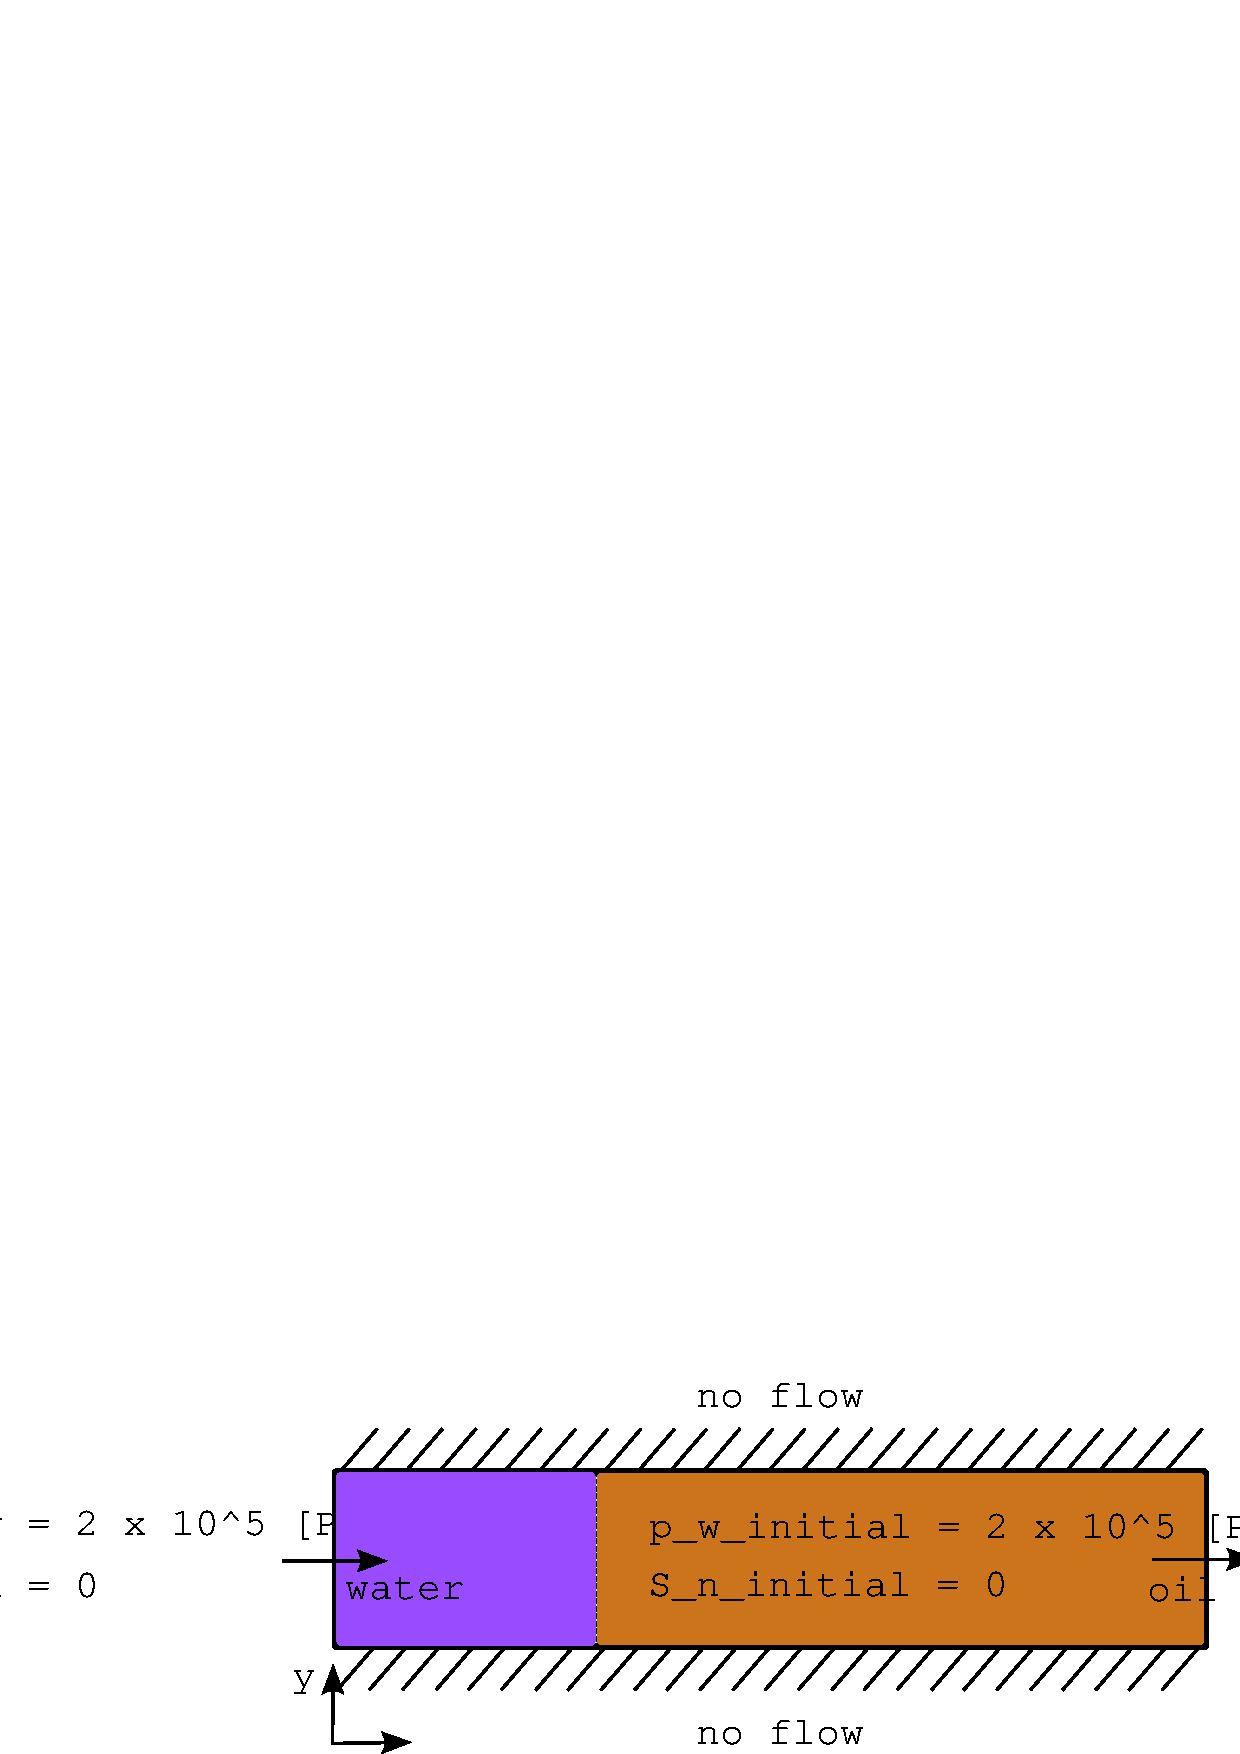
\includegraphics[width=0.9\linewidth,keepaspectratio]{EPS/tutorial-problemconfiguration}
\caption{Geometry of the tutorial problem with initial and boundary conditions.}\label{tutorial-coupled:problemfigure}
\end{figure}

The equations that are solved here are the mass balances of oil and water: \begin{equation}\label{massbalancewater}
\frac {\partial (\phi \, S_{w}\, \rho_{w})}{\partial t} + \nabla \cdot ( \rho_{w} \, \frac{\mathbf{K} \, kr_w}{\mu_{w}} (\nabla p - \rho_{w}\textbf{g})) - q = 0
\end{equation}

\begin{equation}\label{massbalanceoil}
\frac {\partial (\phi \, S_{o}\, \rho_{o})}{\partial t} + \nabla \cdot ( \rho_{o} \, \frac{\mathbf{K} \, kr_o}{\mu_{o}} (\nabla p - \rho_{o}\textbf{g})) - q = 0                                                                      \end{equation}


Listing \ref{tutorial-coupled:mainfile} shows the main file \texttt{tutorial\_coupled.cc} for the coupled twophase model. This file needs to be executed to solve the problem described above. The main file can be found in the directory \texttt{/dune-mux/test/tutorial}.

\begin{lst}[File dune-mux/test/tutorial/tutorial\_coupled.cc]\label{tutorial-coupled:mainfile} \mbox{}
\lstinputlisting[basicstyle=\ttfamily\scriptsize,numbers=left,
numberstyle=\tiny, numbersep=5pt]{../../test/tutorial/tutorial_coupled.cc}
\end{lst}

From line \ref{tutorial-coupled:include-begin} to line \ref{tutorial-coupled:include-end} the Dune and the \Dumux files which contain the functions and classes that are needed in the main function are included into the main file.

The geometry of the problem and the grid on which the problem is to be solved are defined in the lines \ref{tutorial-coupled:grid-begin} to \ref{tutorial-coupled:grid-end}. The three variables of Type \texttt{Dune::FieldVector} define the lower left corner of the domain (\texttt{L}), the upper right corner of the domain (\texttt{H}) and the number of cells in $x$ and $y$ direction (\texttt{N}). The dimension \texttt{dim} is previously defined in line \ref{tutorial-coupled:dim}. The grid of type \texttt{Dune::SGrid} is then generated in line \ref{tutorial-coupled:grid-end}. For more information about the dune grid interface, the different grid types that are supported and the generation of different grids it is referred to the \textit{Dune Grid Interface HOWTO} \cite{DUNE-HP}.

The second step needed to solve the problem is the definition of material properties and constitutive relationships. The fluid properties of the two fluid phases considered here are defined in the lines \ref{tutorial-coupled:water} and \ref{tutorial-coupled:oil}. \Dumux provides several fluid classes which can be found in the file \texttt{phaseproperties2p.hh} in the directory \texttt{/dune-mux/dumux}-\texttt{/material/phaseproperties}. \\
The properties of the solid matrix are defined in a special soil class. The \texttt{soil} object is generated in line \ref{tutorial-coupled:soil}. As can be seen, the class type is \texttt{Dune::TutorialSoil}, which is defined in the file \texttt{tutorial\_soilproperties\_coupled.hh} in the folder \texttt{/test/tutorial}. A description of this file and the definition of a soil class including the soil parameters can be found in section \ref{tutorial-coupled:description-soil-class}. Finally, in line \ref{tutorial-coupled:twophaserelations} the information included in the fluid and soil objects is used to generate an object of type \texttt{Dune::TwoPhaseRelations}, which includes the constitutive relationships (capillary pressure-saturation relation, relative permeability-saturation relation, etc.). The file \texttt{twophaserelations.hh} can be found in the directory \texttt{/dune-mux/dumux/material}.

The definition of boundary and initial conditions as well as source or sink terms is done by definition of a so-called \textit{problem} class. In case of this tutorial the problem class is defined in the file \texttt{tutorialproblem\_coupled.hh} in the \texttt{/test/tutorial} folder. In the main file the problem object of type \texttt{Dune::TutorialProblemCoupled} is then generated in line \ref{tutorial-coupled:problem}. A further explanation of the definition of boundary and initial conditions, source and sink terms and the structure of the problem class can be found in section \ref{tutorial-coupled:description-bc-ic}. Besides the definition of the boundary and initial conditions the problem class is also a kind of interface containing all the objects generated before (geometry, fluids, soil, constitutive relationships, etc.). Thus, as can be seen in line \ref{tutorial-coupled:problem} all this objects are given as arguments when calling the constructor of the problem class.     

Finally, a numerical model has to be chosen that defines how the coupled system of equations is discretized. In case of this tutorial a coupled isothermal two phase model is the choice. A coupled model may consist of two or more mass balance equations and if required an energy balance equation. For the given example problem of a pure isothermal two phase flow. A coupled system of two equations is solved. 
%The two equations are given below:
%\begin{equation}
%\end{equation}
%GLEICHUNGEN\\
%ERKLAERUNG ZU BOX\\

The discretisation of these equations is included in the object which is generated in line \ref{tutorial-coupled:boxmethod} of the main file. It is called \texttt{boxmethod} and it is of type \texttt{Dune::BoxPwSn}. The definition of this class can be found in \texttt{/dune-mux/dumux/twophase/fv} in the file \texttt{boxpwsnjacobian.hh}. The \texttt{Box} in the class name indicates that the \textit{boxmethod} is used for the discretisation. 

Finally, an object called \texttt{timeloop} of type \texttt{Dune::TimeLoop} is generated in line \ref{tutorial-coupled:timeloop} of the tutorial main file. The class \texttt{Dune::TimeLoop} is defined in the file \texttt{timeloop.hh} in the folder \texttt{/dune-mux/dumux/timedisc}. The object \texttt{timeloop} includes the type of timestep that is used (implicit, explicit, etc.) and contains the function \texttt{execute} which is called in line \ref{tutorial-coupled:execute} of the main file. This function finally starts the computation and runs the (time)loop over all timesteps.

\subsection{The definition of the fluid properties}\label{tutorial-coupled:description-fluid-class}

In \Dumux different fluids are already implemented. The definitions can be found in the file \texttt{phaseproperties2p.hh} in the directory \texttt{/dune-mux/dumux/material/phaseproperties}. In this file, for each fluid a class named like the fluid is defined. These classes are derived from the fluid base class \texttt{Fluid} which is defined in the file \texttt{property\_baseclasses.hh} in the directory \texttt{/dune-mux/dumux/material} and include several functions returning different fluid properties. New fluids which are not yet available in the file \texttt{phaseproperties2p.hh} can be defined here accordingly.

It is important to mention, that existing fluid classes should not be changed. New fluid classes should only be added to the file \texttt{phaseproperties2p.hh} if they are also to be added to the repository! If you are not sure if your fluid class can be useful for the other \Dumux users just create a new file in your problem directory similar to the file \texttt{phaseproperties2p.hh} and define your fluid classes there.

\subsection{The definition of the soil parameters}\label{tutorial-coupled:description-soil-class}

Soil properties which can be defined in \Dumux are the \textit{intrinsic permeability}, the \textit{porosity} and the \textit{heat capacity} as well as the \textit{heat conductivity} of the solid matrix. Further the \textit{residual saturations} of the fluids, and the \textit{capillary pressures-saturation function} as well as the \textit{relative permeability-saturation functions} are depending on the soil.

The base class \texttt{Dune::Matrix2p} for the definition of the soil parameters can be found in the file \texttt{property\_baseclasses.hh} in the directory \texttt{/dune-mux/dumux/material}. Derived from this base class, there exist two standard soil type classes named \texttt{HomogeneousSoil} and \texttt{HeterogeneousSoil}. Both can be found in the file \texttt{matrixproperties.hh} in the \texttt{/material} folder. If one wants to use a soil that differs from this standard soil types, new soil classes can be derived either from the base class (\texttt{Dune::Matrix2p}) or from the two standard soil classes (\texttt{Dune::HomogeneousSoil} and \texttt{Dune::HeterogeneousSoil}).

For this tutorial problem a new soil class named \texttt{TutorialSoil} is derived from \texttt{Dune::HomogeneousSoil} (listing \ref{tutorial-coupled:soilpropertiesfile}, line \ref{tutorial-coupled:tutorialsoil}), which can be found in the file \texttt{tutorial\_soilproperties\_coupled.hh} in the directory \texttt{/test/tutorial}.

Listing \ref{tutorial-coupled:soilpropertiesfile} shows the file \texttt{tutorial\_soilproperties\_coupled.hh}.

\begin{lst}[File dune-mux/test/tutorial/tutorial\_soilproperties\_coupled.hh]\label{tutorial-coupled:soilpropertiesfile} \mbox{}
\lstinputlisting[basicstyle=\ttfamily\scriptsize,numbers=left,
numberstyle=\tiny, numbersep=5pt]{../../test/tutorial/tutorial_soilproperties_coupled.hh}
\end{lst}

In line \ref{tutorial-coupled:permeability} the function returning the intrinsic permeability can be found. As can be seen, the function has to be called with three different arguments. The first one (\texttt{x}) is a vector including the global coordinates of the current entity (can be an element, vertex, etc.), the second one (\texttt{e}) is the entity itself and the third one is a vector including the local coordinates of the current entity. The intrinsic permeability is a tensor and thus returned in form of a $n \times n$-matrix where $n$ is the dimension of the problem.

The function \texttt{porosity()} defined in line \ref{tutorial-coupled:porosity} is called with the same arguments as the permeability function described before and returns the porosity dependent on the position in the domain.

The residual saturation functions \texttt{Sr\_w()} (line \ref{tutorial-coupled:srw}) and \texttt{Sr\_n()} (line \ref{tutorial-coupled:srn}) additionally have the temperature as function argument, which is set to a default value if an isothermal model is used.

Finally, the functions defining the type of the capillary pressure function and the relative permeability functions have to be considered. In line \ref{tutorial-coupled:flags} the function \texttt{relPermFlag()} is defined. This function returns a flag indicating the type of function which is used depending on the position. This could be a linear function, a \textit{Brooks-Corey} function, a \textit{van Genuchten} function, etc. The flags that can be chosen as return parameter are defined in the base soil class \texttt{Matrix2p} in the file \texttt{property\_baseclasses.hh}. The parameters used in the chosen function type can be defined in the function \texttt{paramRelPerm} (line \ref{tutorial-coupled:parameters}). As can be seen in listing \ref{tutorial-coupled:soilpropertiesfile}, e.g. linear capillary pressure and relative permeability functions require a vector of two arguments, one defining the minimum and one defining the maximum capillary pressure. The parameters can again be defined depending on the position in the domain an on temperature.

\subsection{The definition of boundary and initial conditions and source or sink terms}\label{tutorial-coupled:description-bc-ic}

Boundary and initial conditions are defined in a so-called problem class. The problem class of this tutorial has the name \texttt{TutorialProblemCoupled} and is defined in the file \texttt{tutorialproblem\_coupled.hh} which can be found in the directory \texttt{/test/tutorial}. Listing \ref{tutorial-coupled:problemfile} shows the class \texttt{TutorialProblemCoupled}. As can be seen it is derived from the problem base class \texttt{TwoPhaseProblem} (line \ref{tutorial-coupled:tutorialproblem}) which is defined in the file \texttt{twophaseproblem.hh} in the directory \texttt{/dune-mux/dumux/twophase}.

\begin{lst}[File dune-mux/test/tutorial/tutorialproblem\_coupled.hh]\label{tutorial-coupled:problemfile} \mbox{}
\lstinputlisting[basicstyle=\ttfamily\scriptsize,numbers=left,
numberstyle=\tiny, numbersep=5pt]{../../test/tutorial/tutorialproblem_coupled.hh}
\end{lst}

Listing \ref{tutorial-coupled:tutorialproblem}) includes five types of functions. The type of each function can be identified by certain letters or names. The function that returns
\begin{itemize}
 \item a source or sink term is called \textbf{q},
 \item a boundary condition type is called \textbf{bctype},
 \item a \textit{Dirichlet} boundary condition is called \textbf{g},
 \item a \textit{Neumann} boundary condition is called \textbf{J} and
 \item an initial condition is called \textbf{initial}.
\end{itemize}

All different function types have to be called with three different arguments. The first one (\texttt{x}) is a vector including the global coordinates of the current entity (can be an element, vertex, etc.), the second
one (\texttt{e}) is the entity itself and the third one is a vector including the local coordinates of the current entity. Thus, the return of the functions, which can be a boundary value, an initial value, a source/sink, etc., can be defined depending on the position in the domain.

The first function defined in the problem class \texttt{TutorialProblemCoupled} is the function \texttt{q} (line \ref{tutorial-coupled:q}). It returns a source or a sink term for the pressure equation.

In line \ref{tutorial-coupled:bctype} the function returning the boundary condition type is defined. 
Flags of type \\
\texttt{Dune::BoundaryConditions::Flags} have to be used as return value of these functions. 
The flags that can be chosen are defined in the file \texttt{boundaryconditions.hh} in the directory \texttt
{/dune-disc/disc/operators}.

In lines \ref{tutorial-coupled:g} the functions returning the \textit{Dirichlet} boundary condition and
in line \ref{tutorial-coupled:J} a function returning the \textit{Neumann} boundary condition are defined.

Finally, the function \texttt{initial} is defined in line \ref{tutorial-coupled:initial}. This function returns the initial values for the pressure and the
saturation.

\subsection{Exercises}
\label{tutorial-coupled:exercises}
The following exercises will give you the opportunity to learn how you can change soil parameters, boundary conditions and fluid properties in \Dumux. For each exercise you can find the output file of the last timestep in the directory \texttt{/dune-mux/dumux/tutorial/results/coupled}.

\subsubsection{Exercise 1}
\renewcommand{\labelenumi}{\alph{enumi})}
For Exercise 1 you only have to make some small changes in the tutorial files.
To get an impression what the results should look like you can first run the original version of the fully-coupled tutorial model by typing  \texttt{./tutorial\_coupled}. For the visualisation with paraview please refer to \ref{quick-start-guide}.
\begin{enumerate}
\item \textbf{Changing the Model Domain and the Boundary Conditions} \\
Change the size of the model domain so that you get a rectangle
with edge lengths of x = 400 m \\  and y = 500 m and with discretisation lengths of  $\Delta \text{x} = 20$ m and $\Delta \text{y} = 20$ m. \\
Change the boundary conditions in the file \texttt{tutorialproblem\_coupled.hh} so that water enters from the bottom and oil is extracted from the top boundary. The right and the left boundary should be closed for water and oil fluxes.  \\
Compile the main file by typing \texttt{make tutorial\_coupled} and run the model.


\item \textbf{Changing Fluids} \\
Now you can change the fluids. Use DNAPL instead of Oil and Brine instead of Water. To do that you have to change the file \texttt{tutorial\_coupled.cc}. If you want to take a closer look how the fluid classes are defined and which fluids are already available please open the file \texttt{phaseproperties2p.hh} in the directory
\texttt{/dune-mux/dumux/material/phaseproperties}.

\item \textbf{Changing Constitutive Relationships} \\
Use a Brooks-Corey law with $\lambda$ = 2 and entry pressure $p_b = 0.0$ instead of a linear law for the relative-permeability/saturation relationship. To do that you have to change the file \texttt{tutorial\_soilproperties\_coupled.hh}. You can find the flag that you have to set for the Brooks-Corey law in the file \texttt{property\_baseclasses.hh} in the directory \texttt{/dune-mux/dumux/material}.  
The available relative permeability and capillary pressure functions are defined in the file \texttt{/dune-mux/dumux/material/relperm\_pc\_law}.
 
\item \textbf{Heterogeneities}  \\
Set up a model domain with the soil properties given in Figure \ref{tutorial-coupled:exercise1_d}. Adjust the boundary conditions so that water is still flowing from the bottom to the top of the domain. You can use the fluids of exercise 1b) and the constitutive relationship of exercise 1c). 

\begin{figure}[h]
\psfrag{K1 =}{K $= 10^{-8}\text{ m}^2$}
\psfrag{phi1 =}{$\phi = 0.15$}
\psfrag{K2 =}{\textcolor{white}{K $= 10^{-9}\text{ m}^2$}}
\psfrag{phi2 =}{\textcolor{white}{$\phi = 0.3$}}
\psfrag{600 m}{600 m}
\psfrag{300 m}{300 m}
\centering
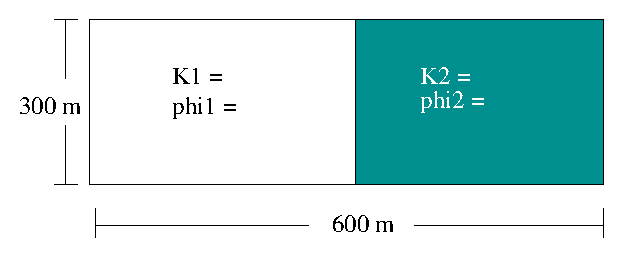
\includegraphics[width=0.5\linewidth,keepaspectratio]{EPS/exercise1_c.eps}
\caption{Exercise 1d: Set-up of a model domain a heterogeneity. $\Delta \text{x} = 20$ m $\Delta \text{y} = 20$ m.}\label{tutorial-coupled:exercise1_d}
\end{figure}

\end{enumerate}

\subsubsection{Exercise 2}
For this exercise you should create a new proplem file according to the file \texttt{tutorialproblem\_coupled.hh} and a new soil property file according to the file \texttt{tutorial\_soilproperties\_coupled.hh}. These files need to be included in the file \texttt{tutorial\_coupled.cc}.\\
The new soil file should contain the definition of a new soil class e.g. SoilEx2. Make sure that you also adjust the preprocessor commands (e.g. change TUTORIAL\_SOILPROPERTIES to TUTORIAL\_SOILEX2). 
The new problem file should contain the definition of a new problem class e.g. ProblemEx2. Here you also need to adjust the preprocessor commands. 
Replace the classes \texttt{TutorialSoil} and \texttt{TutorialProblemCoupled} by the the new classes you just created. \\
Now, set up a model that describes the processes given in the Figures \ref{tutorial-coupled:ex2_Domain} and \ref{tutorial-coupled:ex2_BC}. Initially the domain is fully
saturated with water and the pressure is $p_w = 5 \times 10^5$ Pa. Oil infiltrates from the left side. Create a grid with 20 cells in x direction and 10 cells in y direction. The simulation time should be set to $4\times 10^7$ s.\\
 (Hint: set the maximum time step size to $10^5$ s. This can be done by adding an additional argument when the constructor of the timeloop object is called in the file \texttt{tutorial\_coupled.cc}: \\
\texttt{Dune::TimeLoop<GridType, TwoPhase> timeloop(tStart, tEnd, 100, fileName, modulo,1.e5);})

\begin{figure}[h]
\psfrag{K1}{K $= 10^{-7}\text{ m}^2$}
\psfrag{phi1}{$\phi = 0.2$}
\psfrag{Lin}{Linear Law}
\psfrag{K2}{K $= 10^{-9}\text{ m}^2$}
\psfrag{phi2}{$\phi = 0.15$}
\psfrag{BC1}{Brooks Corey Law} 
\psfrag{BC2}{$\lambda = 1.8$, $p_b = 0.0$}
\psfrag{H1y}{50 m}
\psfrag{H2y}{15 m}
\psfrag{H3y}{20 m}
\psfrag{L1x}{100 m}
\psfrag{L2x}{50 m}
\psfrag{L3x}{25 m}
\centering
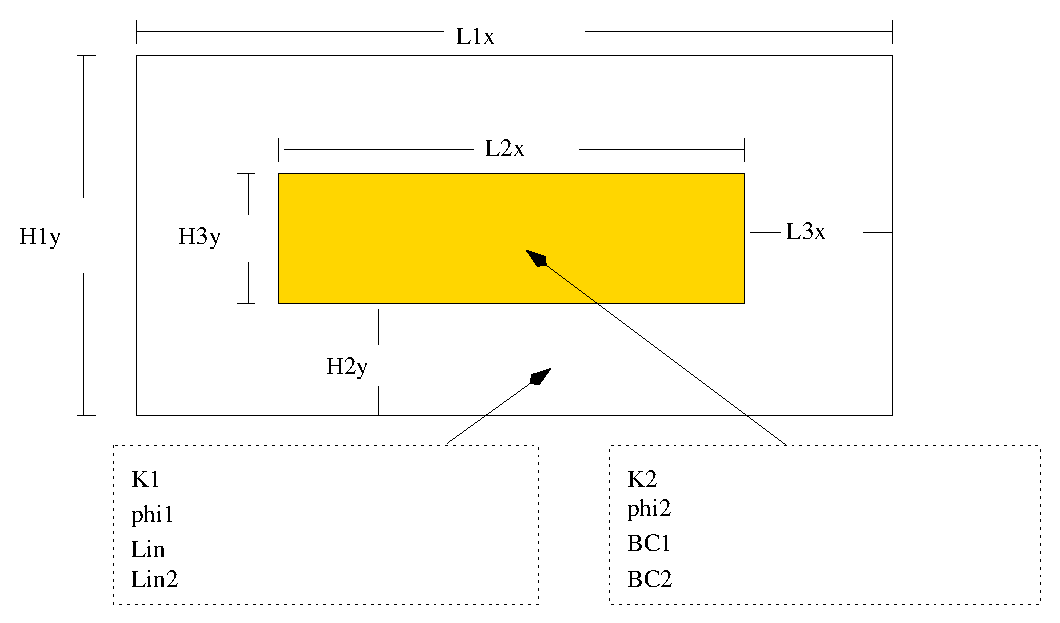
\includegraphics[width=0.8\linewidth,keepaspectratio]{EPS/Ex2_Domain.eps}
\caption{Set-up of the model domain and the soil parameters}\label{tutorial-coupled:ex2_Domain}
\end{figure}

\begin{figure}[h]
\psfrag{pw}{$p_w = 5 \times 10^5$ \text{Pa}}
\psfrag{S}{$S_n = 1.0$}
\psfrag{qw}{$q_w = 2 \times 10^{-4}$ [kg/$\text{m}^2$s]}
\psfrag{qo}{$q_n = 0.0$ [kg/$\text{m}^2$s]}
\psfrag{no flow}{no flow}
\centering
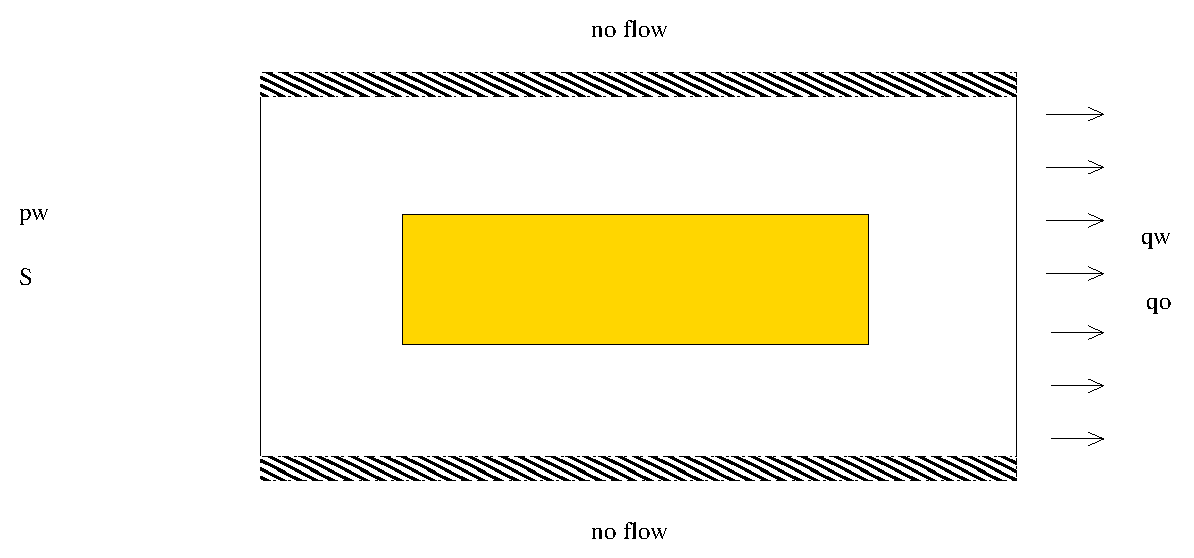
\includegraphics[width=0.8\linewidth,keepaspectratio]{EPS/Ex2_Boundary.eps}
\caption{Boundary Conditions}\label{tutorial-coupled:ex2_BC}
\end{figure}

\subsubsection{Exercise 3}
Create a file called \texttt{new\_fluid.hh} and implement a new fluid class. This new fluid class should be derived from the base class Fluid which can be found in  \texttt{/dune-mux/dumux/material/property\_baseclasses.hh}. \\
(You can look at existing fluid classes in the file \texttt{/dune-mux/dumux/material/phaseproperties/phaseproperties2p.hh}.)
Use methane as a new fluid and run the model of Exercise 2 with water and methane. The properties of methane are given in the following: \\
density: 3.443 kg/$\text{m}^3$, viscosity: 1.0751$\times 10^{-5}$ Pa s. 

\section[Decoupled model]{Solving a problem using a Decoupled Model}\label{tutorial-decoupled}
The process of solving a problem using \Dumux can be roughly divided into four parts: 
\begin{enumerate}
 \item The geometry of the problem and correspondingly a grid have to be defined.
 \item Material properties and constitutive relationships have to be defined.
 \item Boundary conditions as well as initial conditions have to be defined.
 \item A suitable model has to be chosen.
\end{enumerate}

In contrast to the last section, we now apply a decoupled solution procedure, a
so-called \textit{IMPET} (\textit{IM}plicit \textit{P}ressure \textit{E}xplicit 
\textit{T}ransport) algorithm. This means that the pressure equation is first 
solved using an implicit method. The resulting velocities are then used to solve
a transport equation explicitly.\\
In this tutorial, pure fluid phases are solved with a finite volume discretization
of both pressure- and transport step. Primary variables, according to default
settings of the model, are the pressure and the saturation of the wetting phase.

The problem which is solved in this tutorial is illustrated in figure 
\ref{tutorial-decoupled:problemfigure}. A rectangular domain with now flow 
boundaries on the top and at the bottom, which is initially saturated with oil, 
is considered. Water infiltrates from the left side into the domain. Gravity 
effects are neglected.

\begin{figure}[h]
\psfrag{x}{x}
\psfrag{y}{y}
\psfrag{no flow}{no flow}
\psfrag{water}{\textbf{water}}
\psfrag{oil}{\textcolor{white}{\textbf{oil}}}
\psfrag{p_w = 2 x 10^5 [Pa]}{$p_w = 2 \times 10^5$ [Pa]}
\psfrag{p_w_initial = 2 x 10^5 [Pa]}{\textcolor{white}{\textbf{$\mathbf{p_{w_{initial}} = 2 \times 10^5}$ [Pa]}}}
\psfrag{S_n = 0}{$S_w = 1$}
\psfrag{S_n_initial = 0}{\textcolor{white}{$\mathbf{S_{w_{initial}} = 0}$}}
\psfrag{q_w = 0 [kg/m^2s]}{$q_w = 0$ $\left[\frac{\textnormal{kg}}{\textnormal{m}^2 \textnormal{s}}\right]$}
\psfrag{q_n = -3 x 10^-4 [kg/m^2s]}{$q_n = -3 \times 10^-2$ $\left[\frac{\textnormal{kg}}{\textnormal{m}^2 \textnormal{s}}\right]$}
\centering
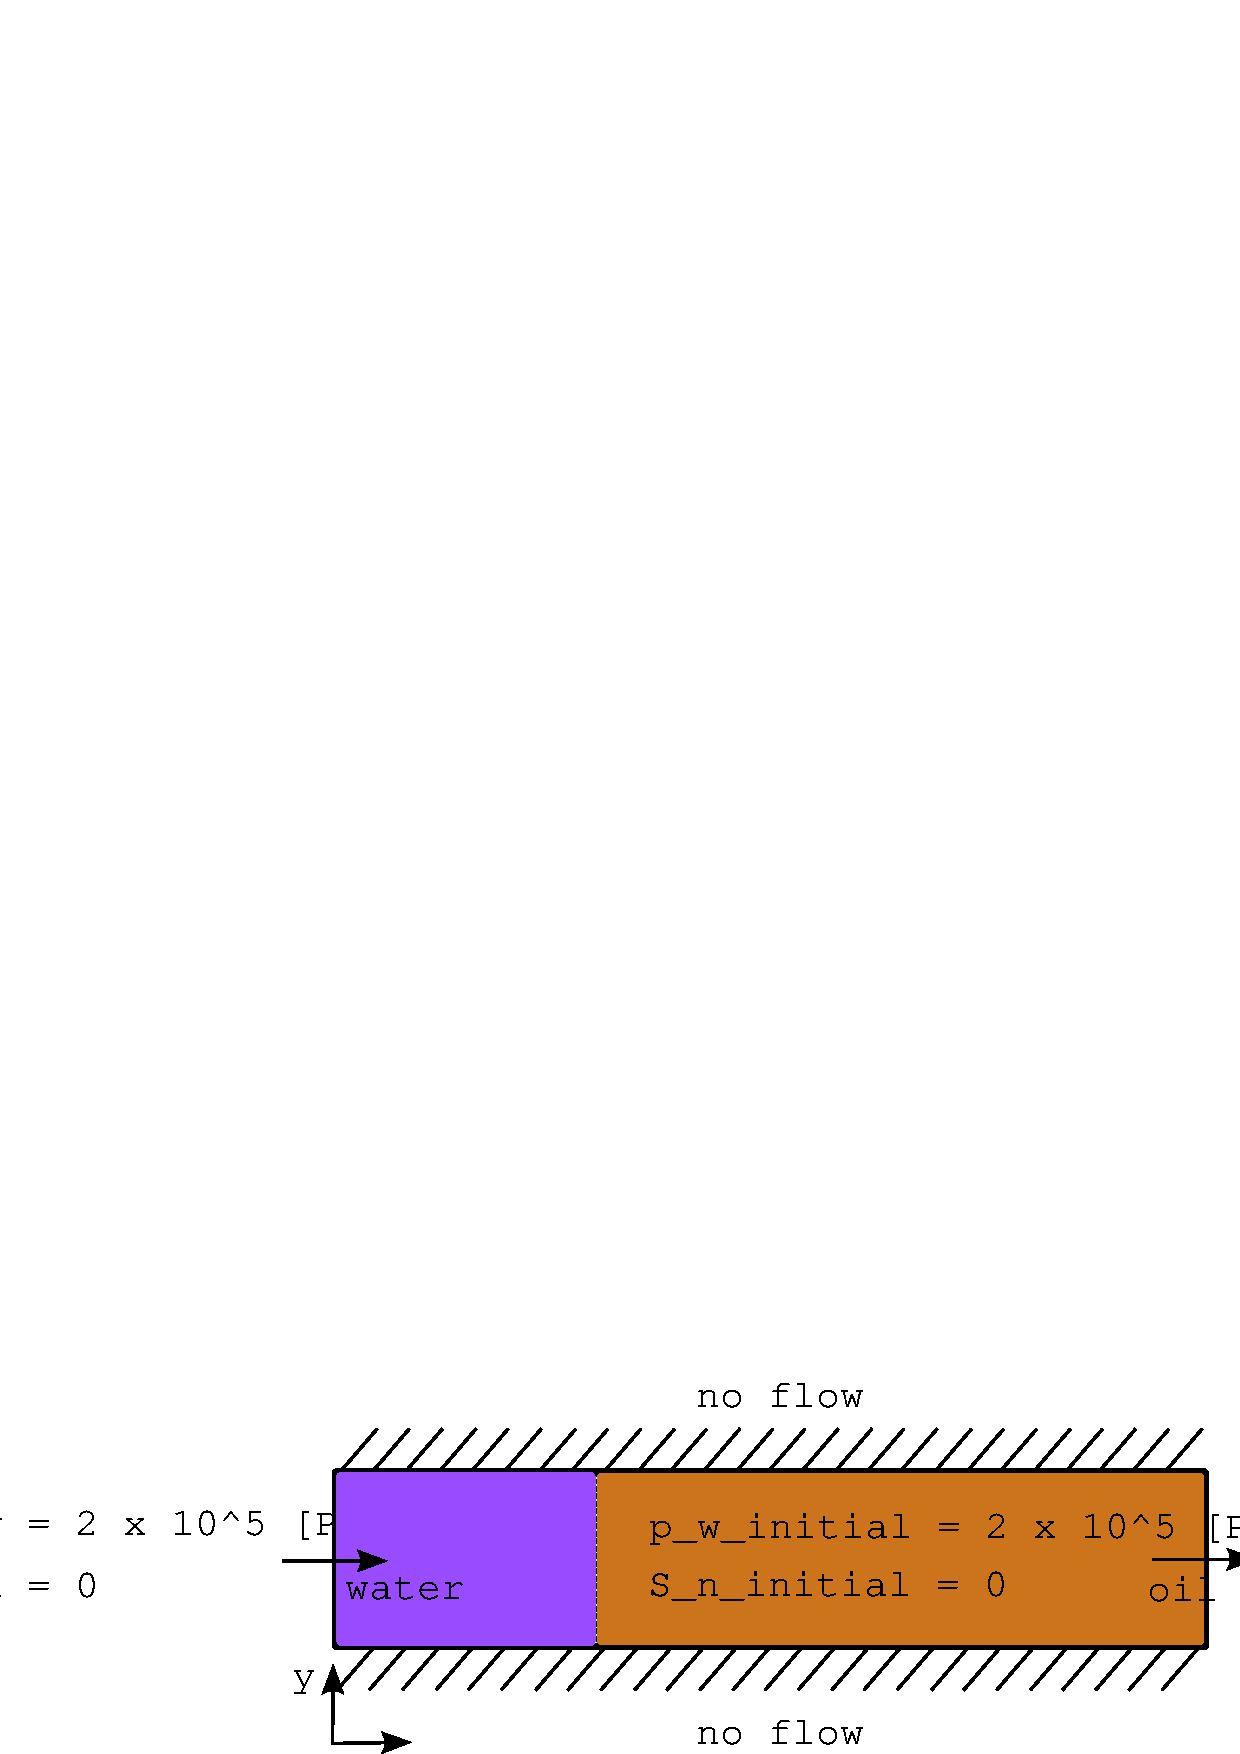
\includegraphics[width=0.9\linewidth,keepaspectratio]{EPS/tutorial-problemconfiguration}
\caption{Geometry of the tutorial problem with initial and boundary conditions.}\label{tutorial-decoupled:problemfigure}
\end{figure}

Listing \ref{tutorial-deoucpled:mainfile} shows how the main file, which has to be executed, has to be set up, if the problem described above is to be solved using a decoupled model. This main file can be found in the directory \texttt{/tutorial} of the stable part of \Dumux.

\begin{lst}[File tutorial/tutorial\_decoupled.cc]\label{tutorial-deoucpled:mainfile} \mbox{}
\lstinputlisting[basicstyle=\ttfamily\scriptsize,numbers=left, 
numberstyle=\tiny, numbersep=5pt]{../../tutorial/tutorial_decoupled.cc}
\end{lst}

First, from line \ref{tutorial-decoupled:include-begin} to line
\ref{tutorial-decoupled:include-end} the \Dune and \Dumux files containing
essential functions and classes are included.

At line \ref{tutorial-decoupled:set-type-tag} the type tag of the
problem which is going to be simulated is set. All other data types
can be retrieved by the \Dumux property system and only depend on this
single type tag. Retrieving them is done between line
\ref{tutorial-decoupled:retrieve-types-begin} and
\ref{tutorial-decoupled:retrieve-types-end}. For an introduction to the
property system, see section \ref{sec:propertysystem}.

The first thing which should be done at run time is to initialize the
message passing interface using \Dune's \texttt{MPIHelper} class. Line
\ref{tutorial-decoupled:init-mpi} line is essential if the simulation is
intended to be run on more than one processor at the same time. Next,
the command line arguments are parsed starting at line
\ref{tutorial-decoupled:parse-args-begin} until line
\ref{tutorial-decoupled:parse-args-end}. In this case, we check if and
at which time a previous run of the simulation should be restarted, and we
parse the time when the simulation ends. As the maximum time-step in the 
sequential model is strictly bound by a CFL-criterion, the first time-step
size is initialized with the simulation time.

After this, a grid is created on line \ref{tutorial-decoupled:create-grid} 
and the problem is instantiated with information about the grid
(via its leaf grid view) on line \ref{tutorial-decoupled:instantiate-problem}.
If demanded, on line \ref{tutorial-decoupled:mainRestart} a state written to
disk by a previous simulation run is restored on request by the user.
Finally, the time manager controlling the simulation run is instantiated 
with the start parameters in line \ref{tutorial-decoupled:initTimeManager}
and the simulation proceedure is started by the time manager at line
\ref{tutorial-decoupled:execute}.



\subsection{The problem class} \label{decoupled_problem}

When solving a problem using \Dumux, the most important file is the
so-called \textit{problem file} as shown in listing
\ref{tutorial-decoupled:problemfile} of
\texttt{tutorialproblem\_decoupled.hh}.

\begin{lst}[File tutorial/tutorialproblem\_decoupled.hh]\label{tutorial-decoupled:problemfile} \mbox{}
\lstinputlisting[basicstyle=\ttfamily\scriptsize,numbers=left,
numberstyle=\tiny, numbersep=5pt, firstline=17]{../../tutorial/tutorialproblem_decoupled.hh}
\end{lst}

First, both \Dune  grid handlers and the decoupled model of \Dumux 
have to be included. Then, a new type tag is created for the problem 
on line \ref{tutorial-decoupled:create-type-tag}.  In this case, the 
new type tag inherits all properties defined for the \texttt{DecoupledTwoP} 
type tag, which means that for this problem the two-phase decoupled approach
is chosen as discretization scheme (defined via the include in line 
\ref{tutorial-decoupled:parent-problem}). On line \ref{tutorial-decoupled:set-problem}, 
a problem class is attached to the new type tag, while the grid which
is going to be used is defined on line \ref{tutorial-decoupled:set-grid-type} --
in this case an \texttt{SGrid} is created.  Since in \Dune, there's no uniform
mechanism to allocate grids, the \texttt{Grid} property also contains
a static \texttt{create()} method which provides just that: From line 
\ref{tutorial-decoupled:grid-begin} to \ref{tutorial-decoupled:grid-end}, 
the geometry is defined and the grid is generated. The three variables of 
Type \texttt{Dune::FieldVector} define the lower left corner of the domain 
(\texttt{L}), the upper right corner of the domain (\texttt{H}) and the number 
of cells in $x$ and $y$ direction (\texttt{N}). The grid of type 
\texttt{Dune::SGrid} is then generated in line \ref{tutorial-decoupled:grid-end}. 
For more information about the \Dune grid interface, the different grid types 
that are supported and the generation of different grids it is referred to 
the \textit{Dune Grid Interface HOWTO} \cite{DUNE-HP}. 

Next, we select the material of the simulation: In case of a pure two-phase
model, each phase is a bulk fluid, and the complex (compositional) fluidsystems
do not need to be used. However, they can be used (see exercise 1 \ref{dec-ex1-fluidsystem}). 
Instead, we use a simplified fluidsystem container that provides classes 
for liquid and gas phases, line \ref{tutorial-decoupled:2p-system-start} to 
\ref{tutorial-decoupled:2p-system-end}. These are linked to the appropriate 
chemical species in line \ref{tutorial-decoupled:wettingPhase} and 
\ref{tutorial-decoupled:nonwettingPhase}. For all parameters that depend 
on space, such as the properties of the soil, the specific spatial parameters 
for the problem of interest are specified in line
\ref{tutorial-decoupled:set-spatialparameters}. 

Now we arrive at some model parameters of the applied two-phase decoupled 
model. Line \ref{tutorial-decoupled:velocityFormulation} defines that the 
wetting phase velocity rather than e.g. a total velocity is used for the 
transport system. As we regard capillary pressure, a capillary diffusive 
term is regarded, selected in line \ref{tutorial-decoupled:DiffusivePart}.
Line \ref{tutorial-decoupled:cfl} assigns the CFL-factor to be used in the
simulation run. The final property on line \ref{tutorial-decoupled:gravity} 
is optional and tells the model not to use gravity.

After all necessary information is written into the property system and 
its namespace is closed in line \ref{tutorial-decoupled:propertysystem-end},
the problem class is defined in line \ref{tutorial-decoupled:def-problem}. 
As its property, the problem class itsself is also derived from a parent, 
\texttt{IMPESProblem2P}. The class constructor (line 
\ref{tutorial-decoupled:constructor-problem}) is able to hold two vectors,
which is not needed in this tutorial.

Besides the definition of the boundary and initial conditions (discussed in 
subsection \label{decoupled-problem:boundary}), the problem class also contains
general information about the current simulation. First, the name used by
the \texttt{VTK-writer} to generate output is defined in the method of line
\ref{tutorial-decoupled:name}, and line \ref{tutorial-decoupled:restart} indicates
weather restart files are written. As decoupled schemes usually feature small 
timesteps, the method controlling the output in line \ref{tutorial-decoupled:output}
is very useful. The divisor of the modulo operation defines after how many timesteps
output should be written out -- the default ``1'' resembles output after each 
step.

The following methods all have in common that they may be dependent on space.
Hence, they all feature a common argument list:
\begin{itemize}
 \item \texttt{globalPos}: A vector holding the global Coordinates.
 \item \texttt{element} or \texttt{intersection}: Input for an iterator, that is 
    depending weather the parameter of the method is defined in an element, such as 
    initial values, or on an intersection, such as a boundary condition.
\end{itemize}
In the following, there are the methods for general parameters, source- or
sinkterms, boundary conditions (lines \ref{tutorial-decoupled:bctypePress} to
\ref{tutorial-decoupled:neumann}) and initial values for the transported
quantity in line \label{tutorial-decoupled:initSat}. For more information
on the functions, it is referred to the documentation in the code.

\subsection{The definition of the parameters that are dependent on space}\label{tutorial-decoupled:description-spatialParameters}

Listing \ref{tutorial-decoupled:spatialparametersfile} shows the file
\verb+tutorialspatialparameters_decoupled.hh+:

\begin{lst}[File tutorial/tutorialspatialparameters\_decoupled.hh]\label{tutorial-decoupled:spatialparametersfile} \mbox{}
\lstinputlisting[basicstyle=\ttfamily\scriptsize,numbers=left,
numberstyle=\tiny, numbersep=5pt, firstline=16]{../../tutorial/tutorialspatialparameters_decoupled.hh}
\end{lst}
As this file only slightly differs from the coupled version, it is referred to 
chapter \ref{tutorial-coupled:description-spatialParameters} for explanations.
However, as a standard Finite-Volume--scheme is used, in contrast to the box-method
in the coupled case, the argument list here is the same as for the problem 
functions:
\begin{itemize}
 \item \texttt{globalPos}: A vector holding the global Coordinates.
 \item \texttt{element}: Input for an element iterator, providing access
	to the current element of interest.
\end{itemize}

\subsection{Exercise}
\label{tutorial-deoucpled:exercises}
The following exercises will give you the opportunity to learn how you can change 
soil parameters, boundary conditions and fluid properties in \Dumux and to play along 
with the decoupled modelling framework.

\subsubsection{Exercise 1}
\renewcommand{\labelenumi}{\alph{enumi})}
For Exercise 1 you only have to make some small changes in the tutorial files.
\begin{enumerate}
\item \textbf{Altering output}
To get an impression what the results should look like you can first run the original version of the decoupled tutorial model by typing  \texttt{./tutorial\_decoupled 1e5}. The number behind the simulation name defines the timespan of the simulation run in seconds. For the visualisation with paraview please refer to \ref{quick-start-guide}.\\
As you can see, the simulation creates roughly 150 output files. To reduce these to perform longer simulations, change the method responsible for output in the file \texttt{tutorialproblem\_decoupled} to write an output only every 20 timesteps. Compile the main file by typing \texttt{make tutorial\_decoupled} and run the model. Now, run the simulation for 5e5 seconds.

\item \textbf{Changing the Model Domain and the Boundary Conditions} \\
Change the size of the model domain so that you get a rectangle
with edge lengths of x = 300 m \\  and y = 300 m and with discretisation lengths of  $\Delta \text{x} = 20$ m and $\Delta \text{y} = 10$ m. \\
Change the boundary conditions in the file \texttt{tutorialproblem\_decoupled.hh} so that water enters from the bottom and oil flows out at the top boundary. The right and the left boundary should be closed for water and oil fluxes.  \\

\item \textbf{Changing Fluids} \\
Now you can change the fluids. Use DNAPL instead of Oil and Brine instead of Water. To do that you have to select different components via the property system in the problem file:
\begin{enumerate}
 \item Brine: The class \texttt{Dumux::Brine} acts as a adapter to the fluid system that alters a pure water class by adding some salt. Hence, the class \texttt{Dumux::Brine} uses a pure water class, such as \texttt{Dumux::H2O}, as a second template argument after the data type \texttt{<Scalar>} as a template argument (be aware to use the complete water class with its own template parameter).
 \item DNAPL: A standard set of chemical substances is already included (via a list of \texttt{\#include ..} commandos) and hence easy accessible by default. This is not the case for the class \texttt{Dumux::SimpleDNAPL}, however, which is located in the folder \texttt{dumux/material/components/}. Try to include the file as well as select the component via the property system.
\end{enumerate}
If you want to take a closer look how the fluid classes are defined and which substances are already available please browse through the files in the directory
\texttt{/dumux/material/components}.

\item \textbf{Use the \Dumux fluid system}\label{dec-ex1-fluidsystem} \\
As you have experienced in the coupled tutorial (chapter \ref{tutorial-decoupled}), \Dumux usually organises fluid mixtures via a \texttt{fluidsystem}. This is also possible for the decoupled models: Uncomment, as we want to reuse it later on, the lines \ref{tutorial-decoupled:2p-system-start} to \ref{tutorial-decoupled:2p-system-end} in the problem file. If you use eclipse, this can easily be done by pressing \textit{str + shift + 7}, the same shortcut works to cancel the comment later on.\\
Now include the file \texttt{fluidsystems/h2o\_n2\_system.hh} in the material folder, and set a property \texttt{FluidSystem} with the appropriate type, \texttt{Dumux::H2O\_N2\_System<TypeTag>}. However, the complicated fluidsystem uses tabularized fluid data, which need to be initialized in the constructor body of the current problem by adding \texttt{GET\_PROP\_TYPE(TypeTag, PTAG(FluidSystem))::init();}, hence using the initialization function of the applied fluidsystem. As an alternative, use a simpler version of water, e.g. \texttt{Dumux::SimpleH2O}, and apply it for the property \texttt{Components} with type \texttt{H2O}. The density of the gas is magnitudes smaller than that of oil, so please decrease the injection rate to $q_n = -3 \times 10^-4$ $\left[\frac{\textnormal{kg}}{\textnormal{m}^2 \textnormal{s}}\right]$. Also reduce the simultation duration to 1e5 seconds.\\
Please reverse the changes of this example, as we still use bulk phases and hence do not need such an extensive fluid system.
 
\item \textbf{Heterogeneities}  \\
Set up a model domain with the soil properties given in Figure \ref{tutorial-deoucpled:exercise1_d}. Adjust the boundary conditions so that water is again flowing from left to right.
\begin{figure}[h]
\psfrag{K1 =}{K $= 10^{-8}\text{ m}^2$}
\psfrag{phi1 =}{$\phi = 0.15$}
\psfrag{K2 =}{\textcolor{white}{K $= 10^{-9}\text{ m}^2$}}
\psfrag{phi2 =}{\textcolor{white}{$\phi = 0.3$}}
\psfrag{600 m}{600 m}
\psfrag{300 m}{300 m}
\centering
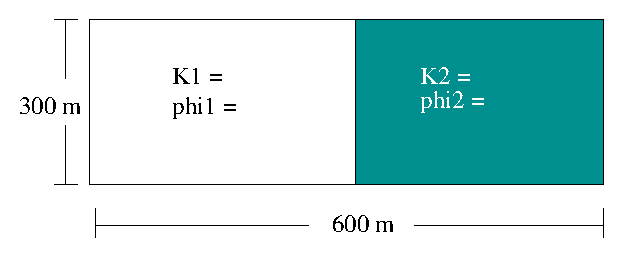
\includegraphics[width=0.5\linewidth,keepaspectratio]{EPS/exercise1_c.eps}
\caption{Exercise 1d: Set-up of a model domain a heterogeneity. $\Delta \text{x} = 20$ m $\Delta \text{y} = 20$ m.}\label{tutorial-deoucpled:exercise1_d}
\end{figure}
When does the front cross the material border? In paraview, the option \textit{View} $\rightarrow$ \textit{Animation View} is nice to get a rough feeling of the timestep sizes.
\end{enumerate}

\subsubsection{Exercise 2}
For this exercise you should create a new proplem file analogous to
the file \texttt{tutorialproblem\_decoupled.hh} and new spatial parameters 
just like \texttt{tutorialspatialparameters\_decoupled.hh}. These files need to
be included in the file \texttt{tutorial\_decoupled.cc}. 

The new file defining spatial parameters should contain the definition 
of a new class, such as \texttt{SpatialParametersEx2}. Make sure that you also adjust the guardian
macros in the header files (e.g. change \texttt{TUTORIALSPATIALPARAMETERS\_COUPLED} to
\texttt{SPATIALPARAMETERSEX2}). Besides also adjusting the guardian macros, 
the new problem file should define and use a new type tag for the problem as well as a new problem class
e.g. \texttt{ProblemEx2}. Make sure you assign your newly defined spatial 
parameter class to the \texttt{SpatialParameters} property for the new 
type tag. 

After this, change the \texttt{create()} method of the \texttt{Grid}
property so that it matches the domain described
by figure \ref{tutorial-decoupled:ex2_Domain}. Adapt the problem class
so that the boundary conditions are consistent with figure
\ref{tutorial-decoupled:ex2_BC}. Initially the domain is fully saturated
with water and the pressure is $p_w = 2 \times 10^5 \text{Pa}$ . Oil
infiltrates from the left side. Create a grid with $20$ cells in
$x$-direction and $10$ cells in $y$-direction. The simulation time
should be set to $1e5 \text{s}$.

Now include your new problem file in the main file and replace the
\texttt{TutorialProblemCoupled} type tag by the one you've created and
compile the program.


\begin{figure}[h]
\psfrag{K1}{K $= 10^{-7}\text{ m}^2$}
\psfrag{phi1}{$\phi = 0.2$}
\psfrag{Lin}{Brooks Corey Law} 
\psfrag{Lin2}{$\lambda = 1.8$, $p_b = 100$}
\psfrag{K2}{K $= 10^{-9}\text{ m}^2$}
\psfrag{phi2}{$\phi = 0.15$}
\psfrag{BC1}{Brooks Corey Law} 
\psfrag{BC2}{$\lambda = 2$, $p_b = 500$}
\psfrag{H1y}{50 m}
\psfrag{H2y}{15 m}
\psfrag{H3y}{20 m}
\psfrag{L1x}{100 m}
\psfrag{L2x}{50 m}
\psfrag{L3x}{25 m}
\centering
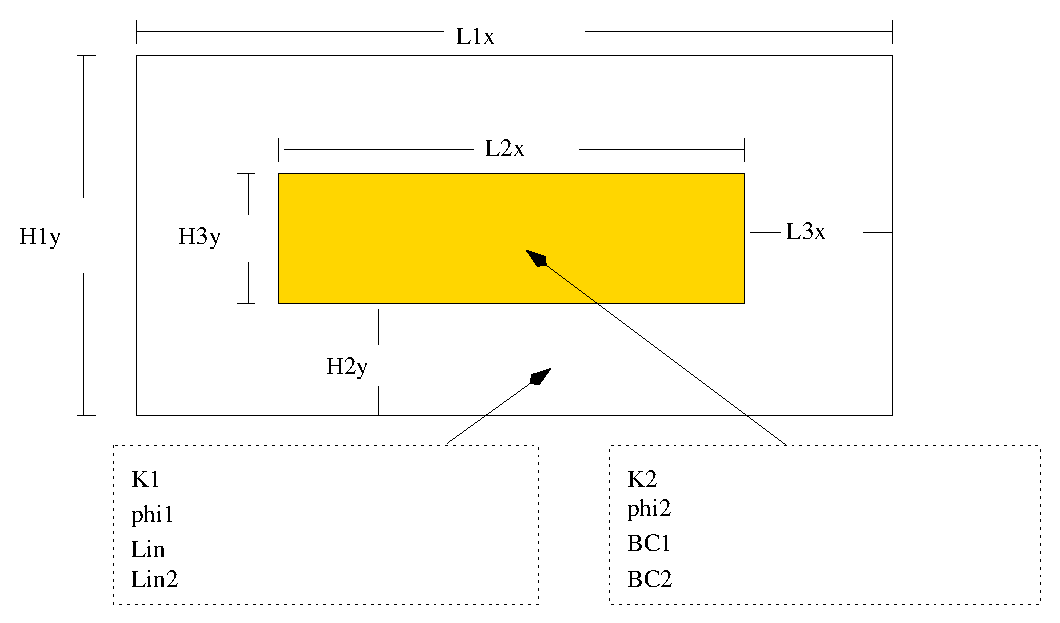
\includegraphics[width=0.8\linewidth,keepaspectratio]{EPS/Ex2_Domain.eps}
\caption{Set-up of the model domain and the soil parameters}\label{tutorial-decoupled:ex2_Domain}
\end{figure}

\begin{figure}[h]
\psfrag{pw}{$p_w = 2 \times 10^5$ [\text{Pa}]}
\psfrag{S}{$S_w = 0.0$}
\psfrag{qw}{$q_w = 3 \times 10^{-4}$ [kg/$\text{m}^2$s]}
\psfrag{qo}{$q_n = 0.0$ [kg/$\text{m}^2$s]}
\psfrag{no flow}{no flow}
\centering
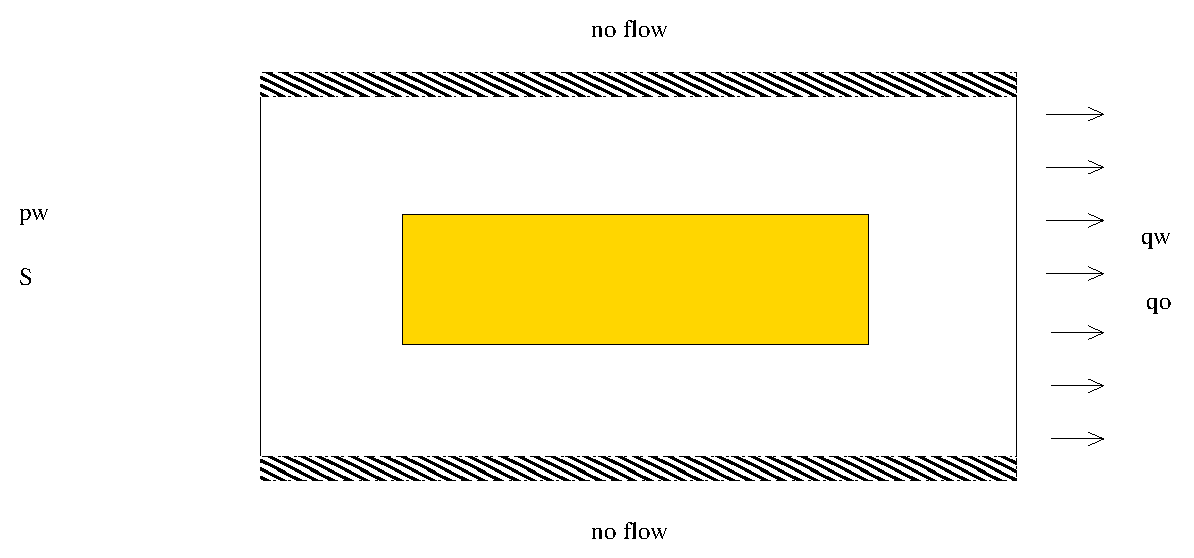
\includegraphics[width=0.8\linewidth,keepaspectratio]{EPS/Ex2_Boundary.eps}
\caption{Boundary Conditions}\label{tutorial-decoupled:ex2_BC}
\end{figure}

\begin{itemize}
 \item What happens if you increase the resolution of the grid? Hint: Paraview can visualize the timesteps via the ``Animation View'' (to be enabled unter the button \textit{View}).
 \item Set the CFL-factor to 1 and investigate the saturation: Is the value range reasonable?
 \item Further increase the CFL-factor to 2 and investigate the saturation.
\end{itemize}


\subsubsection{Exercise 3}
Create a new file for benzene called \texttt{benzene.hh} and implement
a new fluid system. (You may get a hint by looking at existing fluid 
systems in the directory \verb+/dumux/new_material/fluidsystems+.)

Use benzene as a new fluid and run the model of Exercise 2 with water
and benzene. Benzene has a density of $889.51 \, \text{kg} / \text{m}^3$
and a viscosity of $0.00112 \, \text{Pa} \; \text{s}$. 

%%% Local Variables: 
%%% mode: latex
%%% TeX-master: "dumux-handbook"
%%% End: 

%\section[New model]{How to implement a new model}

TODO: describe how to impelment a new model

\bibliographystyle{plain}
\bibliography{dumux-handbook}

\printindex

\end{document}
